\documentclass[prb,aps,twocolumn,floatfix,amsmath,amssymb,superscriptaddress,tightenlines]{revtex4}
\usepackage{graphicx}
\usepackage{epstopdf}
\usepackage{amsfonts}
\usepackage{bm}
\usepackage{color}
\usepackage{ulem}
\newcommand{\be}{\begin{equation}}
\newcommand{\ee}{\end{equation}}
\begin{document}

\subsection{Valence Bond Quantum Monte Carlo}

This algorithm, pioneered by Sandvik \cite{papers} in 2005, is a ground state projection monte carlo technique performed in the valence bond basis.

A high power of the Hamiltonian $\mathcal{H}^m$ 
is applied to a trial state, projecting out the ground state of the system.
We use the Heisenberg Hamiltonian, which is rewritten in terms of bond operators $(H_{ab} = \tfrac{1}{4} - {\bf S}_a \cdot {\bf S}_b)$ acting on pairs of sites.
The Hamiltonian can be written as a sum of all possible {permutations (with repetition)} of these bond operators.
The Monte Carlo algorithm samples terms proportional to their weight in the sum, where the weight depends on the number of off-diagonal operators in the term.

This scheme can be used to project out one copy of the groundstate wavefunction (single projector) or simultaneously project two copies (double projector) which can be used to measure expectation values of observables in the simulation. 

\subsubsection{Loop Algorithm}

\begin{figure} {
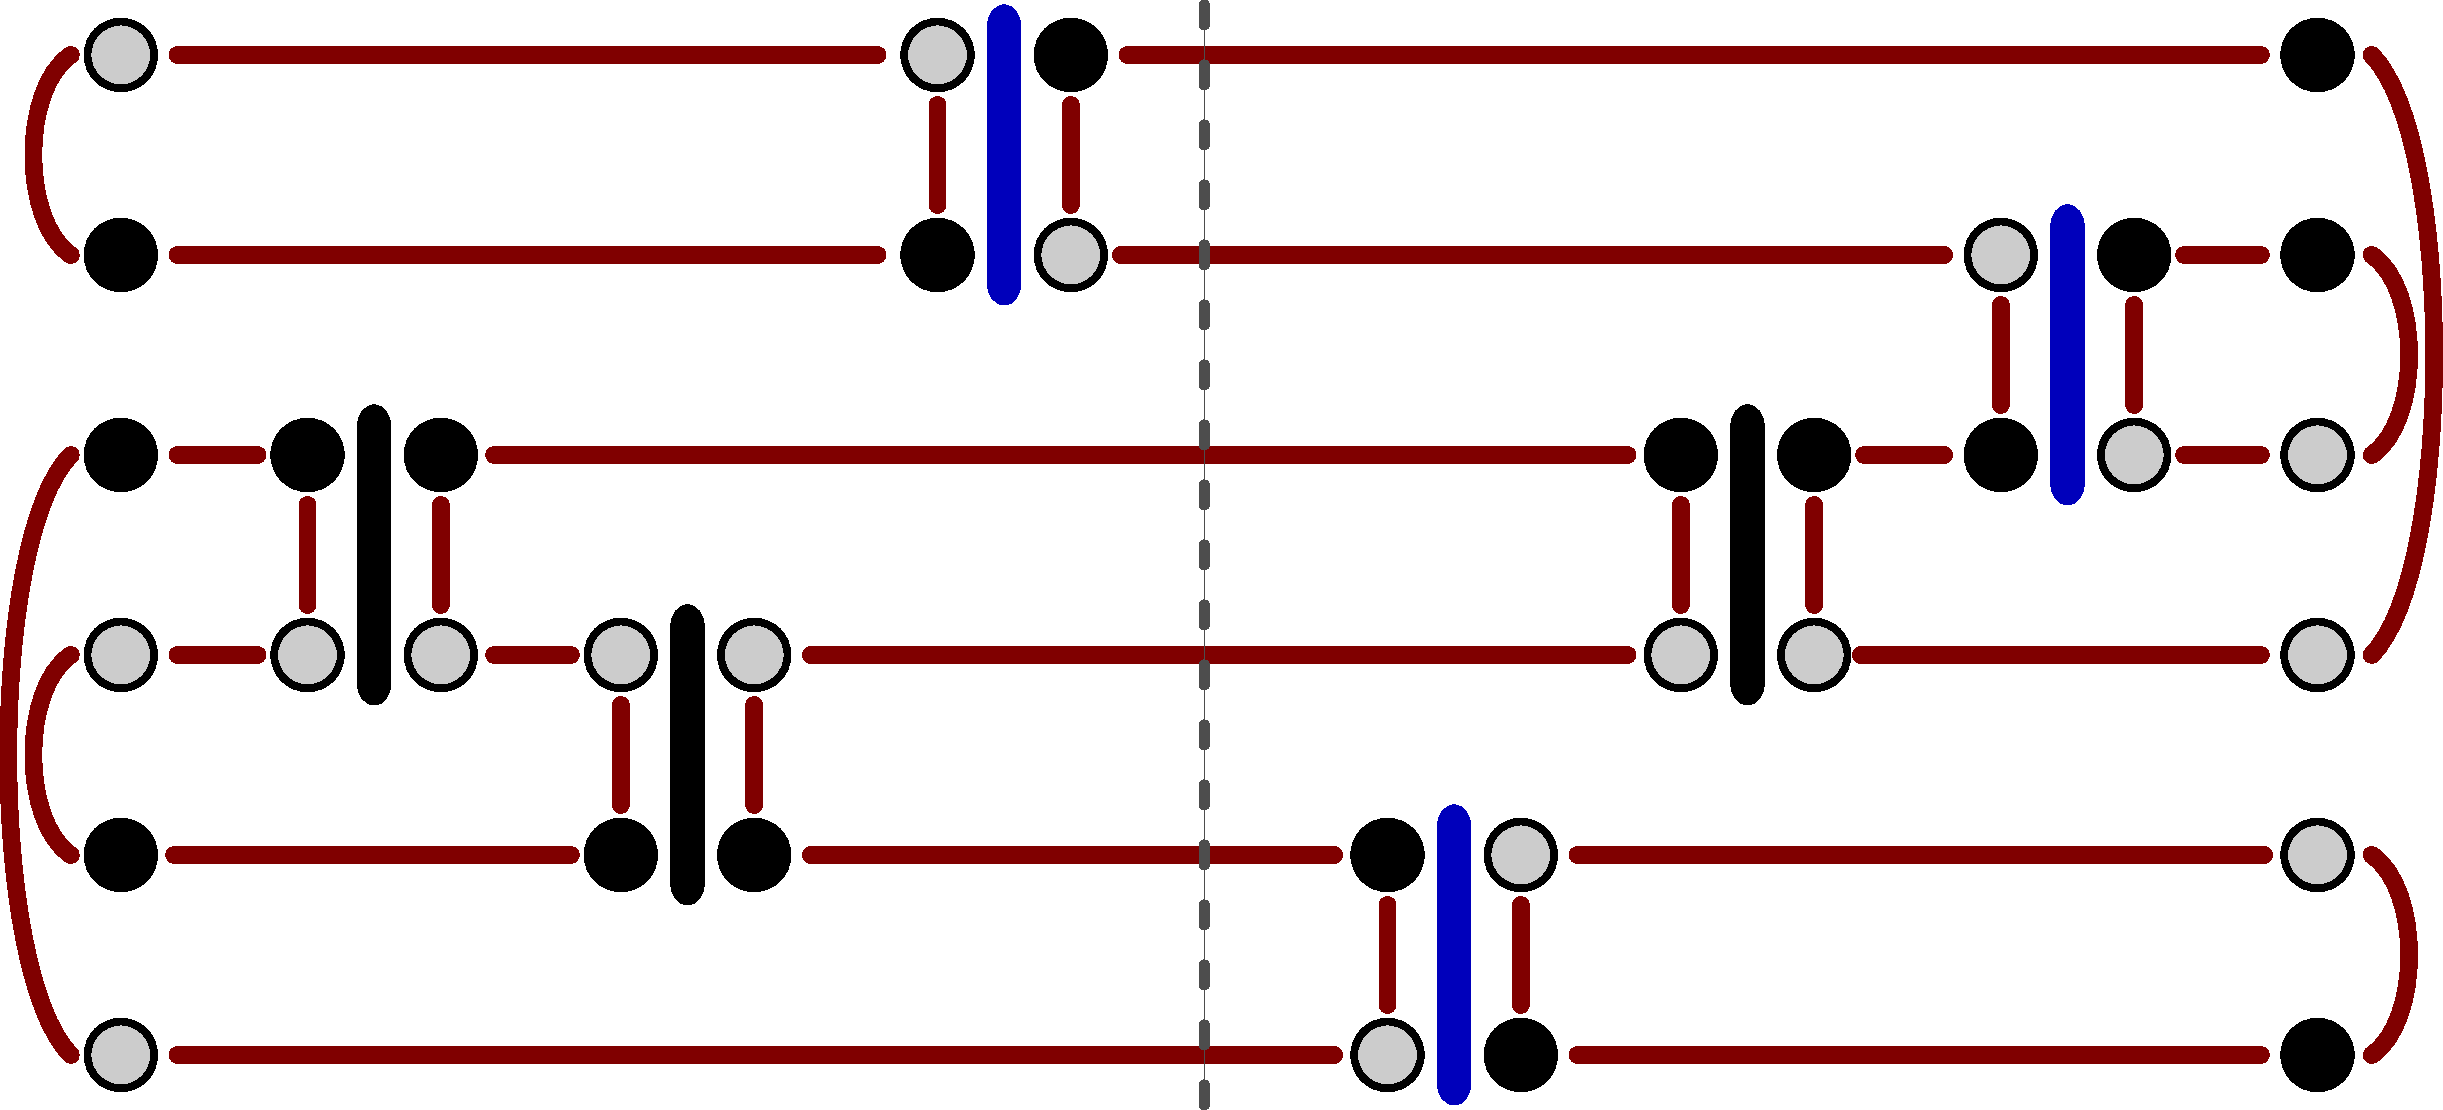
\includegraphics[width=3.2 in]{loopalg.pdf} \caption{ A possible VB-spin-operator diagram for a 6-site system.
Up (down) spins are shown in grey (black). (Off-)diagonal operators are shown in (blue) black.
\label{loop1} }
} \end{figure}

In addition to valence bonds this scheme samples over spin states, eliminating the need for a rejection step, and thus sampling operators and states more efficiently.

The operators in this case are divided into two classes,
\begin{eqnarray}
	H_{ab}(1) &=&(\tfrac{1}{4} - S^z_aS^z_b) \\
	H_{ab}(2) &=& %-(S_a^xS_b^x + S_a^yS_b^y). 
		         -\tfrac{1}{2}(S_a^+S_b^- + S_a^-S_b^+)
\end{eqnarray}
called diagonal and offi-diagonal operators respectively, where the sum $H_{ab}(1) + H_{ab}(2)$ is equal to the bond operators $H_{ab}$ from the standard VB QMC algorithms mentioned above.

The algorithm is best visualized using a VB-spin-operator diagram, as shown in Figure \ref{loop1}.
Along with the trial VB states (shown on the left and right edges of the figure) initial spin states are also selected at random, with the condition that the two spins in a single VB must be antiparallel.
For each trial state $m$ operators are chosen (initially all diagonal operators), such that they are all acting on pairs of antiparallel spins.
There are two types of updates in this algorithm: spin updates and operators updates.

For the spin update, the loops generated by the operators and valence bonds are each ``flipped'' with probability $1/2$, so that every spin in the loop is flipped.
This update samples possible spin states for the given valence bond configuration.

In the second type of update the operators are changed so that all remaining diagonal operators and reselected randomly, such that they are still acting on antiparallel sites.
This reconfigures the propagated valence bond states.

Measurements can be computed as usual using the propagated valence bond states, $\lvert V_L \rangle$ and $\lvert V_R \rangle$ which can be extracted from the VB-spin-operator diagram by following the loops crossing the dotted line in figure \ref{loop1}.


%\noindent
%-trial states... along with spin states.\\
%-m operators are picked for each trial state to act on antiparallel spins\\
%-VB-spin-operator diagram with loops and stuff\\
%- loop *and* operator update\\
%-loop spins flipped with prob 1/2 (sample over possible spin states)..\\
%-only diagonal operators changed (why)\\
%-projected state(s) are at the centre of vb-spin-operator diagram, can be used for measurements.\\
%- similar to SSE\\

\subsection{Measuring the Renyi Entanglement Entropies using VB QMC}
%mention measurement in SSE too!
Entanglement entropy is difficult to measure in QMC because we do not have direction access to the groundstate wavefunction of the system.
However, methods to measure entanglement have been developed and implemented in {\color{red} several} types of Monte Carlo simulations ({\color{red} refs}).

\subsubsection{The Renyi Entropies}
The Renyi entropies are used to quantify entanglement between a system subdivided into two regions, $A$ and $B$.
They are defined as 
\begin{equation} \label{renyi}
S_{\alpha}(A) = \frac{1}{1-\alpha}\ln \left[ {\rm Tr}(\rho_A^{\alpha}) \right],
\end{equation}
where $\rho_A = {\rm Tr}_B (\rho)$ is the reduced density matrix of the total system traced out over region $B$.\\
%talk about the von Neumann EE in the limit of $\alpha \rightarrow 1$?

\subsubsection{The Swap Operator}
%reference to swap paper... and cardy?
Despite not having access to the wavefunction of the system on Monte Carlo techniques, it is possible to sample ${\rm Tr}(\rho_A^{\alpha})$ for integer $\alpha > 1$.
This is accomplished by taking the expectation value of a $Swap$ operator, %swap paper
or permutation operator for $\alpha > 2$.% cardy paper


To measure the $\alpha^{\rm th}$ entropy each projected state must include $\alpha$ non-interacting copies of the system.
These permutation operators $\Pi_\alpha^A$ operators act to cyclicly exchange the state in region $A$ between different copies of the system, and are constructed such that  $\langle \Pi_\alpha^A \rangle = {\rm Tr}(\rho_A^{\alpha})$.
In the case of spin states, which are all product states in our simulations, we can simply swap the states within the region $A$s.  
For valence bond states the application of the permutation operator also has a simple result; it acts to exchange the endpoints of valence bonds within region $A$ between copies of the system, and so can create bonds between the copies.

The bare measurement of the $Swap$ operator has been shown ({\color{red} refs}) to have problems with convergence for large region $A$, while in principle it should be symmetric such that $\langle Swap_A \rangle = \langle Swap_B \rangle$.
This is because the exchange of a larger region gives a larger number of different states as a result of that swap, and thus a larger range and number of possible values in the expectation value.
It simply takes more Monte Carlo steps to converge upon the same result.


\subsubsection{The Ratio Trick}
This convergence issue has been addressed by a reweighting of the Monte Carlo sampling.

In the double projector method we measure the expectation value by sampling terms from 
\be
\langle \mathcal{O} \rangle =\frac {\sum_{lr} w_r w_r\langle V_l  \lvert V_r\rangle\frac{  \langle V_l  \lvert \mathcal{O} \lvert V_r\rangle}{ \langle V_l  \lvert V_r\rangle}}
		{\sum_{lr} w_l w_r \langle V_l  \lvert V_r\rangle}
\ee
where $\lvert V_l \rangle, \lvert V_r \rangle$ are the states obtained by applying lists of bond operators to the trial states and $w_l , w_r $ are the weights accrued by applying those operators.
Terms are sampled proportional to the total weight $W = w_l w_r \langle V_l  \lvert V_r\rangle$, by accepting a new configuration with probability $W^{\rm new}/W^{\rm old}$.
Thus we can simply measure $\tfrac{  \langle V_l  \lvert \mathcal{O} \lvert V_r\rangle}{ \langle V_l  \lvert V_r\rangle}$ periodically, and the average value will give us $\langle \mathcal{O} \rangle$.

%make this all for permutation operator instead?
For the {\it ratio trick}, we modify the weight to include the expectation value of a $Swap$ operator for a region $A$ that is close in size to the region we intend to measure.  
We then measure the ratio of these two operators, e.g.
\be
\frac{\langle {Swap_{A}} \rangle}{\langle {Swap_{A'}} \rangle} =\frac {\sum_{lr} w_r w_r\langle V_l \lvert Swap_{A'} \lvert V_r\rangle\frac{  \langle V_l  \lvert Swap_A \lvert V_r\rangle}{ \langle V_l \lvert Swap_{A'} \lvert V_r\rangle}}
		{\sum_{lr} w_l w_r \langle V_l \lvert Swap_{A'} \lvert V_r\rangle}.
\ee
This improves the sampling because, if regions $A$ and $A'$ are similar in size, the measurement $\tfrac{  \langle V_l  \lvert Swap_A \lvert V_r\rangle}{ \langle V_l \lvert Swap_{A'} \lvert V_r\rangle}$ will have fewer possible values than $\tfrac{  \langle V_l  \lvert Swap_A \lvert V_r\rangle}{ \langle V_l \lvert V_r\rangle}$, and those values will be in a smaller range.

We are, however, only measuring a {\it ratio} of expectation values.
To obtain $ \langle Swap_A \rangle $ we must know the value of $ \langle Swap_{A'} \rangle $.
So, to measure the entropies for a range of sizes of region $A$ we can begin with a measurement of the bare $Swap$ for a small region size and increase the size of regions $A$ and $A'$ over several simulations.
Though we can measure any region $A$ within a simulation, we can only use one size of  $A'$ per simulation because it affect the sampling of the valence bond states.


%- normally sampled with weight including overlap <vL | vR> \\
%- modified so it's <vL | Swap | vR>




\subsection{The Loop Ratio Algorithm for VB QMC}

\begin{figure} {
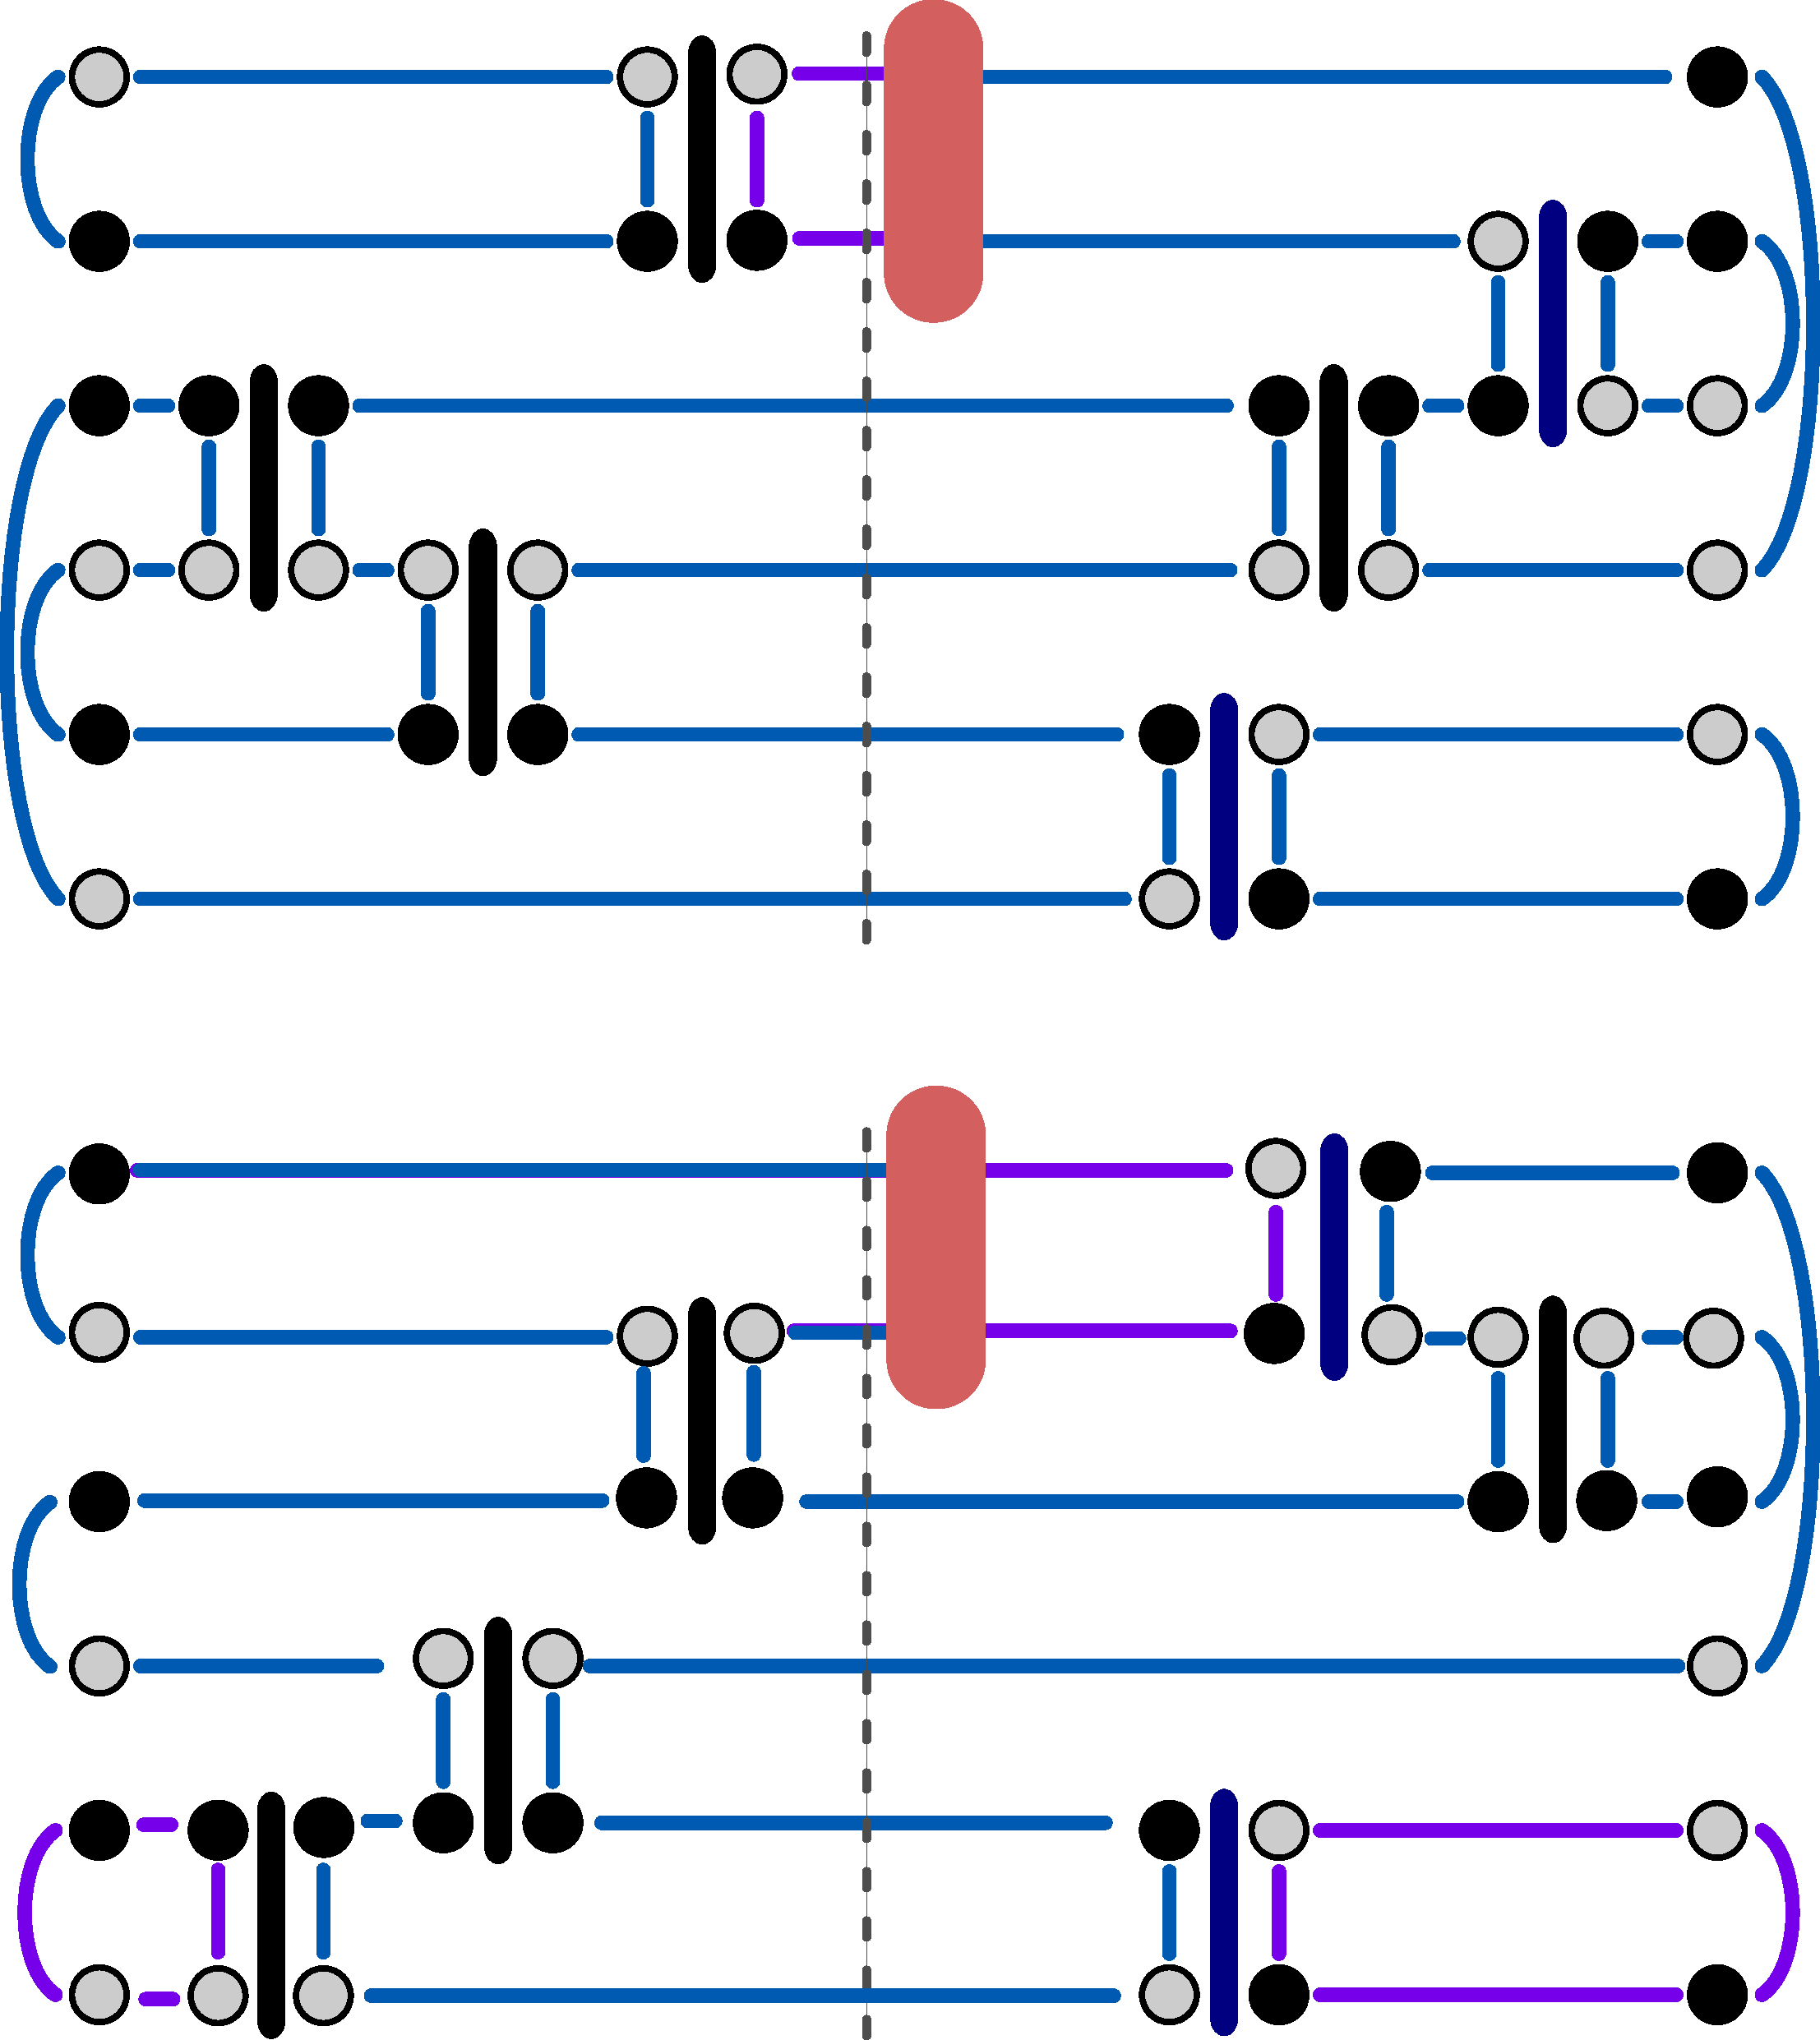
\includegraphics[width=3.2 in]{loopalgratio.pdf} \caption{ 
\label{lratio} %A possible VB-spin-operator diagram for a 4-site system with m=2 operators per copy of the system, {\bf (something about ratio and used to calculate the 2nd renyi entropy)
%(also, make sure the two copies have *different* operators and loops, but still compatible spin configurations)}
The VB-spin-operator diagram for to loop ratio algorithm on a 6-site system where $\alpha =2$ and region $A'$ contains the first 2 sites of the system.
Spins between the usually non-interacting copies are connected through loops via the $Swap$ operator.
}
} \end{figure}

The same principles apply when modifying the loop algorithm to use the ratio trick, however the sampling weight is less apparent in this scheme because we instead sample over spin states whose overlap is always 1.

The main modification to the algorithm is a reconnection of the links in the VB-spin-operator list as if there were a $Swap$ operator permanently applied to the projected state $\lvert V_r \rangle$, shown for $\alpha = 2$ in figure \ref{lratio}.
This causes spins from different non-interacting copies of the system to be connected via loops, which means they can be flipped together, and thus the spin states are sampled according to the swapped system $\langle V_l  \lvert Swap_{A'} \lvert V_r\rangle$.
The measurement of  $\langle V_l  \lvert Swap_{A} \lvert V_r\rangle/\langle V_l  \lvert Swap_{A'} \lvert V_r\rangle$ is then accomplished by measuring an operator which swaps the states of the sites in region $A$ that were not already swapped in region $A'$, assuming $A' \subset A$.

This method possesses the same limitation of the double projector ratio trick, that only one value of $A'$ can be used per simulation, so the region measure must be built up from a small region $A$.


%- multiple copies... 
%- reconnection of the links as if a swap operator was applied
%- affects the sampling of the spin states...

\end{document}
